\section{Results} \label{sect:3}

In this section I will present the results of the evaluation of \eqref{eq:prox_nonneg(prox_r)} and \eqref{eq:prox_r(prox_nonneg)}, for \textit{simple} regularizers (e.g. norms acting on the raw arrays) to more complex, state-of-the-art image regularizers. In these cases, I will also present some experiments on standard test images. A summary of the results is presented in Table \ref{tab:exp_results}.

\begin{center}
    \begin{table}[H]
    \begin{tabular}{||c|c|c|c|c|c||}
        \hline
        %%%%%%%%%%%%%%%%%%%%%% HEADING %%%%%%%%%%%55
        Dimension & $\mathbf{L}$ & $\operatorname{R}$ & $\mathrm{prox}_{\delta}(\mathrm{prox}_{\mathcal{R}}(\mathbf{v}))$ & $\mathrm{prox}_{\mathcal{R}}(\mathrm{prox}_{\delta}(\mathbf{v}))$ & Parameters \cr 
        \hline \hline
        
        %%%%%%%%%%%%%%%%%%%%55 PReviousely Known casesw %%%%%%%
        1, 2 & $\operatorname{I}$ & $\|\cdot\|_1$ &  \checkmark ($10^{-5}$)& \checkmark ($10^{-7}$) & $\mathcal{N}(0, 1)$, $x\in \mathbb{R}^{100}$\\ 
        1, 2 & $\operatorname{I}$ &  $\|\cdot\|_2$ & $\times$($10^{-3}$)& \checkmark ($10^{-6}$)&$\mathcal{N}(0, 1)$, $x\in \mathbb{R}^{100}$\cr \hline
        
        %%%%%%%%%%%% Identity 
        1, 2 & $\operatorname{I}$ &  $\|\cdot\|_p$ & $\times$($10^{-3}$) & \checkmark ($10^{-7}$) & $\mathcal{N}(0, 1)$, $x\in \mathbb{R}^{100}$\\
        1, 2 & $\operatorname{I}$ & $\|\cdot\|_p^p$ & \checkmark ($10^{-6}$) & \checkmark ($10^{-6}$) & $\mathcal{N}(0, 1)$, $x\in \mathbb{R}^{100}$\\
        2 & $\operatorname{I}$ & $\|\cdot\|_{S_1}$ &  $\times$ ($10^{-2}$) & $?$ ($10^{-3}$) & $\mathcal{N}(0, 100)$, $x\in \mathbb{R}^{2 \times 2}$ \\
        2 & $\operatorname{I}$ & $\|\cdot\|_{S_2}$ &  $\times$ ($10^{-2}$) & $?$ ($10^{-3}$) & $\mathcal{N}(0, 100)$, $x\in \mathbb{R}^{2 \times 2}$ \\
        2 & $\operatorname{I}$ & $\|\cdot\|_{S_3}$ &  $\times$ ($10^{-2}$) & $?$ ($10^{-3}$) & $\mathcal{N}(0, 100)$, $x\in \mathbb{R}^{2 \times 2}$\cr\hline
        
        %%%%%%%%%%%% Total Viariation 
        1 & $\nabla_1$ & $\|\cdot\|_1$ & \checkmark ($10^{-6}$)& $\times$ ($10^{-1}$) & $\mathcal{N}(0, 1)$, $x\in \mathbb{R}^{50}$ \\
        1 & $\nabla_1$ & $\|\cdot\|_p$ & $\times$ ($10^{-2}$) & $\times$ ($10^{-2}$) & $\mathcal{N}(0, 1)$, $x\in \mathbb{R}^{50}$\\
        1 & $\nabla_1$ & $\|\cdot\|_p^p$ & $\times$ ($10^{-2}$) & $\times$ ($10^{-2}$) & $\mathcal{N}(0, 1)$, $x\in \mathbb{R}^{50}$ \\
        2 & $\nabla_2$ & $\|\cdot\|_{1, 1}$ &  \checkmark ($10^{-7}$)& $\times$ ($10^{-1}$) & $\mathcal{N}(0, 1)$, $x\in \mathbb{R}^{40\times 40}$\\
        2 & $\nabla_2$ & $\|\cdot\|_{p, q}$ & $\times$ ($10^{-2}$)& $\times$ ($10^{-1}$) & $\mathcal{N}(0, 1)$, $x\in \mathbb{R}^{40\times 40}$\\
        2 & $\nabla_2$ & $\|\cdot\|_{p, q}^{p, q}$ & $\times$ ($10^{-1}$)& $\times$ ($10^{-1}$) & $\mathcal{N}(0, 1)$, $x\in \mathbb{R}^{40\times 40}$\cr \hline
        
        %%%%%%%%%%%%%%%%%%%%%%%%%% Group Sparsity
        1, 2 &  $\operatorname{I}$ & $\|\cdot\|_{1, 1}$  & \checkmark ($10^{-7}$) & \checkmark ($10^{-7}$) & $\mathcal{N}(0, 1)$, $x\in \mathbb{R}^{40 \times 40}$\\
        1, 2 &  $\operatorname{I}$ & $\|\cdot\|_{p, q}$  & $\times$ ($10^{-2}$)& \checkmark ($10^{-6}$) & $\mathcal{N}(0, 1)$, $x\in \mathbb{R}^{40 \times 40}$\\
        1, 2 &  $\operatorname{I}$ & $\|\cdot\|_{p, q}^{p, q}$  & $\times$ ($10^{-4}$)& \checkmark ($10^{-7}$) & $\mathcal{N}(0, 1)$, $x\in \mathbb{R}^{40 \times 40}$\\
        1, 2 &  $\operatorname{I}$ & $\|\cdot\|_{1, q}$  &  \checkmark ($10^{-7}$)& \checkmark ($10^{-7}$) & $\mathcal{N}(0, 1)$, $x\in \mathbb{R}^{40 \times 40}$ \\
        1, 2 &  $\operatorname{I}$ & $\|\cdot\|_{p, 1}^{p, q}$  &  \checkmark ($10^{-7}$) & \checkmark ($10^{-7}$) & $\mathcal{N}(0, 1)$, $x\in \mathbb{R}^{40 \times 40}$ 
        \cr \hline
        
        %%%%%%%%%%%%%%%%%%%%%%%%%% Hessian Schatten + DCT
        % 1 & $\operatorname{DCT}$ &  $\ell_1$ & $\times$& $\times$ & \cr\hline
        % 2 & $\operatorname{HS}$ & $\ell_*$ & Seems & $\times$ &\\
        2 & $\operatorname{HS}$ & $\|\cdot\|_{S_1, p}$ &  $\times$ ($10^{-1}$) & $\times$ ($10^{-1}$) & $\mathcal{N}(0, 10)$, $x\in \mathbb{R}^{15 \times 15}$\\ 
        2 & $\operatorname{HS}$ & $\|\cdot\|_{S_2, p}$ &  $\times$ ($10^{-1}$) & $\times$ ($10^{-1}$) & $\mathcal{N}(0, 10)$, $x\in \mathbb{R}^{15 \times 15}$\\
        2 & $\operatorname{HS}$ & $\|\cdot\|_{S_{\infty}, p}$ &  $\times$ ($10^{-1}$) & $\times$ ($10^{-1}$) & $\mathcal{N}(0, 10)$, $x\in \mathbb{R}^{15 \times 15}$ \cr\hline
    \end{tabular}
    \caption{\label{tab:exp_results} Experimental Results. The first three columns describe the regularizer $\mathcal{R}$, while the fourth and fifth columns present the results obtained with the average absolute error. The last column shows the parameters used to obtain the presented results. In all cases, $100$ different arrays were sampled and tested, and the average absolute error is presented over the hundred samples. The first two rows show results that were previously known, and are therefore useful to test the setup of the project. The rest of the lines separate the table by transform applied to the original signal/image. The second block corresponds to simple norms, the third block to $\operatorname{TV}$ regularizers, the fourth one to Group Sparsity regularizers and the fifth block to Hessian-Schatten norm regularizers.}
    \end{table}
\end{center}

As explained in section \ref{sect:2environment}, I used CVXPy to evaluate all image regularizers, constructing them in terms of combinations of simple convex functions. In particular, for the derivatives needed to calculate $\operatorname{TV}$ and the Hessian-Schatten norm, I used only the valid region of the resulting array, to avoid boundary artifacts. 

\noindent\textbf{$\ell_1$, $\ell_2$ norm} 

The $\ell_1$ and $\ell_2$ norms were studied with the purpose of validating the experimental setup, as these results are already known in the literate \cite{del_aguila_pla_cell_2018}. Moreover, as presented in section \ref{sect:prox_solutions}, and depicted in figure \ref{fig:prox_closed_form_sols}, there is a closed-form solution. However, I still used the experimental setup as a validation of the methodology. 

As shown in table \ref{tab:exp_results}, the results agree with the literature. In the case of the $\ell_1$ norm, both \eqref{eq:prox_nonneg(prox_r)} and \eqref{eq:prox_r(prox_nonneg)} are valid for $\mathcal{R} = \ell_1$, with average absolute errors in the order of $10^{-5}$ for  \eqref{eq:prox_r(prox_nonneg)} and of $10^{-7}$ for  \eqref{eq:prox_nonneg(prox_r)}. In the case of $\mathcal{R} = \ell_2$, I also recovered the results presented in \cite{del_aguila_pla_cell_2018}. I found that  \eqref{eq:prox_r(prox_nonneg)} is valid with average absolute errors in the order of $10^{-6}$, while  \eqref{eq:prox_nonneg(prox_r)} does not hold true, with average absolute errors in the order of $10^{-3}$. 

This error rates, applied on simple regularizers and with $1$-dimensional and $2$-dimensional, reasonably big arrays, provide guidelines on what I will consider to validate or not equations \eqref{eq:prox_nonneg(prox_r)} and \eqref{eq:prox_r(prox_nonneg)}.

\noindent\textbf{$\ell_p$ and $\ell_p^p$ norms} 

After validating the experimental methodology, I made an investigation of the $\ell_p$ norm (for $p \in \mathbb{Z}^+$). The results show that the properties found in \cite{del_aguila_pla_cell_2018, del_aguila_pla_cell_2018-1} for the $\ell_2$ norm can be generalized, which means that any norm of the $\ell_p$ norm family - where $p$ is a positive integer- satisfies  \eqref{eq:prox_r(prox_nonneg)}, with average absolute errors in the order of $10^{-7}$. 

Following the previous results and looking at how both  \eqref{eq:prox_r(prox_nonneg)} and  \eqref{eq:prox_nonneg(prox_r)} hold true for the $\ell_1$ norm (a particular case where $\ell_p^p$ = $\ell_p$), I looked further at the family of norms $\ell_p^p$. The results are very promising, as I found that both \eqref{eq:prox_r(prox_nonneg)} and  \eqref{eq:prox_nonneg(prox_r)} hold true for all $\ell_p^p$ norms. Moreover, all average absolute errors are in the order of $10^{-6}$, an error comparable to the one found for the $\ell_1$ and $\ell_2$ norms. 

\noindent\textbf{Schatten Norms}

While they are not used as image regularizers by themselves, I also studied the family of Schatten Norms for $p \in \{1, 2, \infty\}$, mostly motivated by their use in the Hessian-Schatten norm. I studied different combinations of parameters (matrices of sizes ranging from $2\times 2$ to $20\times 20$, Gaussian distributions with $\sigma$ in the range $[0, 100]$), and in every case got similar results to the ones presented in table \ref{tab:exp_results}. In the results I show, the ratio $\frac{\sigma}{\epsilon}$ (where $\epsilon$ is the average absolute error) is high enough to suggest that the Schatten (for $p \in \{1, 2, \infty\}$) norm might fulfill  \eqref{eq:prox_r(prox_nonneg)}, and encouraging enough to study the Hessian-Schatten image regularizer. However, the experimental setup used in this project is unable to arrive to a definitive conclusion, and a close-form study should be done.  

As discussed in Section \ref{sect:2evaluating}, in general, bigger arrays have lower error rates. In this regard, the Schatten norms are the first functions to have a computational limitation, as the results presented were taken on arrays much smaller than the arrays used to evaluate $\ell_p$. This is because evaluating the Schatten norm of larger matrices involves expensive singular value computations, and it was unfeasible to perform an experiment of the same size as the one performed for the $\ell_p$ norm. Therefore, I arrive to the conclusion that further study is required to determine the results for the Schatten norm.

\noindent\textbf{Group Sparsity}

The evaluation of group sparsity was done over both $1$-dimensional and $2$-dimensional arrays. As presented in table \ref{tab:exp_results}, the results were the same in both cases, which is completely expected since we are taking $p$-norms, and the dimensionality of the array does not play a role. The average absolute errors are in the order of $10^{-7}$ for the cases that I judged satisfactory. In particular, in every single studied case (all possible combinations of $\|\cdot\|_{p, q}$ and $\|\cdot\|_{p, q}^{p, q}$, where $\|\cdot\|_{p, q}^{p, q}$ stands for taking an inner $\ell_p^p$ and an outer $\ell_q^q$ norm ),  \eqref{eq:prox_r(prox_nonneg)} holds true. This was expected from the previous results found on norms, and even though not every single case of  \eqref{eq:prox_nonneg(prox_r)} holds true, as explained in section \ref{sect:1} only one of both equations is required to avoid splitting during reconstruction. This encourages the use of group sparsity as regularizer, as there are no particular conditions to be met during its use to allow for reduced splitting. 

\noindent\textbf{Total Variation} 

As described in section \ref{sect:2regularizers}, $\operatorname{TV}$ is a regularizer of utmost importance in the signal and image processing fields. For the $1$-dimensional cases, following the results previously presented, I studied $\mathcal{R} = \|\operatorname{D}\mathbf{x}\|_p$ and $\mathcal{R} = \|\operatorname{D}\mathbf{x}\|_p^p$. As table \ref{tab:exp_results} shows, only the case of $\mathcal{R} = \|\operatorname{D}\mathbf{x}\|_1$ makes  \eqref{eq:prox_nonneg(prox_r)} valid, with an average absolute error in the order of $10^{-6}$. On all the other cases ($\mathcal{R} = \|\operatorname{D}\mathbf{x}\|_p$, and $\mathcal{R} = \|\operatorname{D}\mathbf{x}\|_p^p$, both for $p \in \mathbb{Z}^+ \backslash\{1\}$), average absolute errors are in the order of $10^{-2}$, which demonstrate that neither of \eqref{eq:prox_nonneg(prox_r)} and \eqref{eq:prox_r(prox_nonneg)} hold true. 

In the case of $2$-dimensional arrays or images, the results obtained are very similar results. I tried several combinations of the $\|\cdot\|_{p, q}$ and the $\|\cdot\|_{p, q}^{p, q}$ mixed norms. Table \ref{tab:exp_results} shows that only the combination $p = 1$ and $q = 1$ satisfies  \eqref{eq:prox_nonneg(prox_r)}, with average absolute errors in the order of $10^{-7}$. As mentioned in section \ref{sect:2regularizers}, this combination is known as nonisotropic $\operatorname{TV}$ and it is a well known, widely used regularizer. The rest of the combinations show average absolute errors in the range of $[10^{-1}, 10^{-3}]$, depending on the combination. 

To further explore the nonisotropic $\operatorname{TV}$ (the explicit expression is given in \eqref{eq:tv11} and, as explained above, has several desirable properties, with  \eqref{eq:prox_nonneg(prox_r)} being an additional one), I decided to test on a toy image. I choose the Shepp-Logan phantom, as it is a standard test image composed of piece-wise constant segments, so it is optimal for exemplifying the effects of $\operatorname{TV}$ minimization. 

\begin{figure}[H]
  \begin{center}
  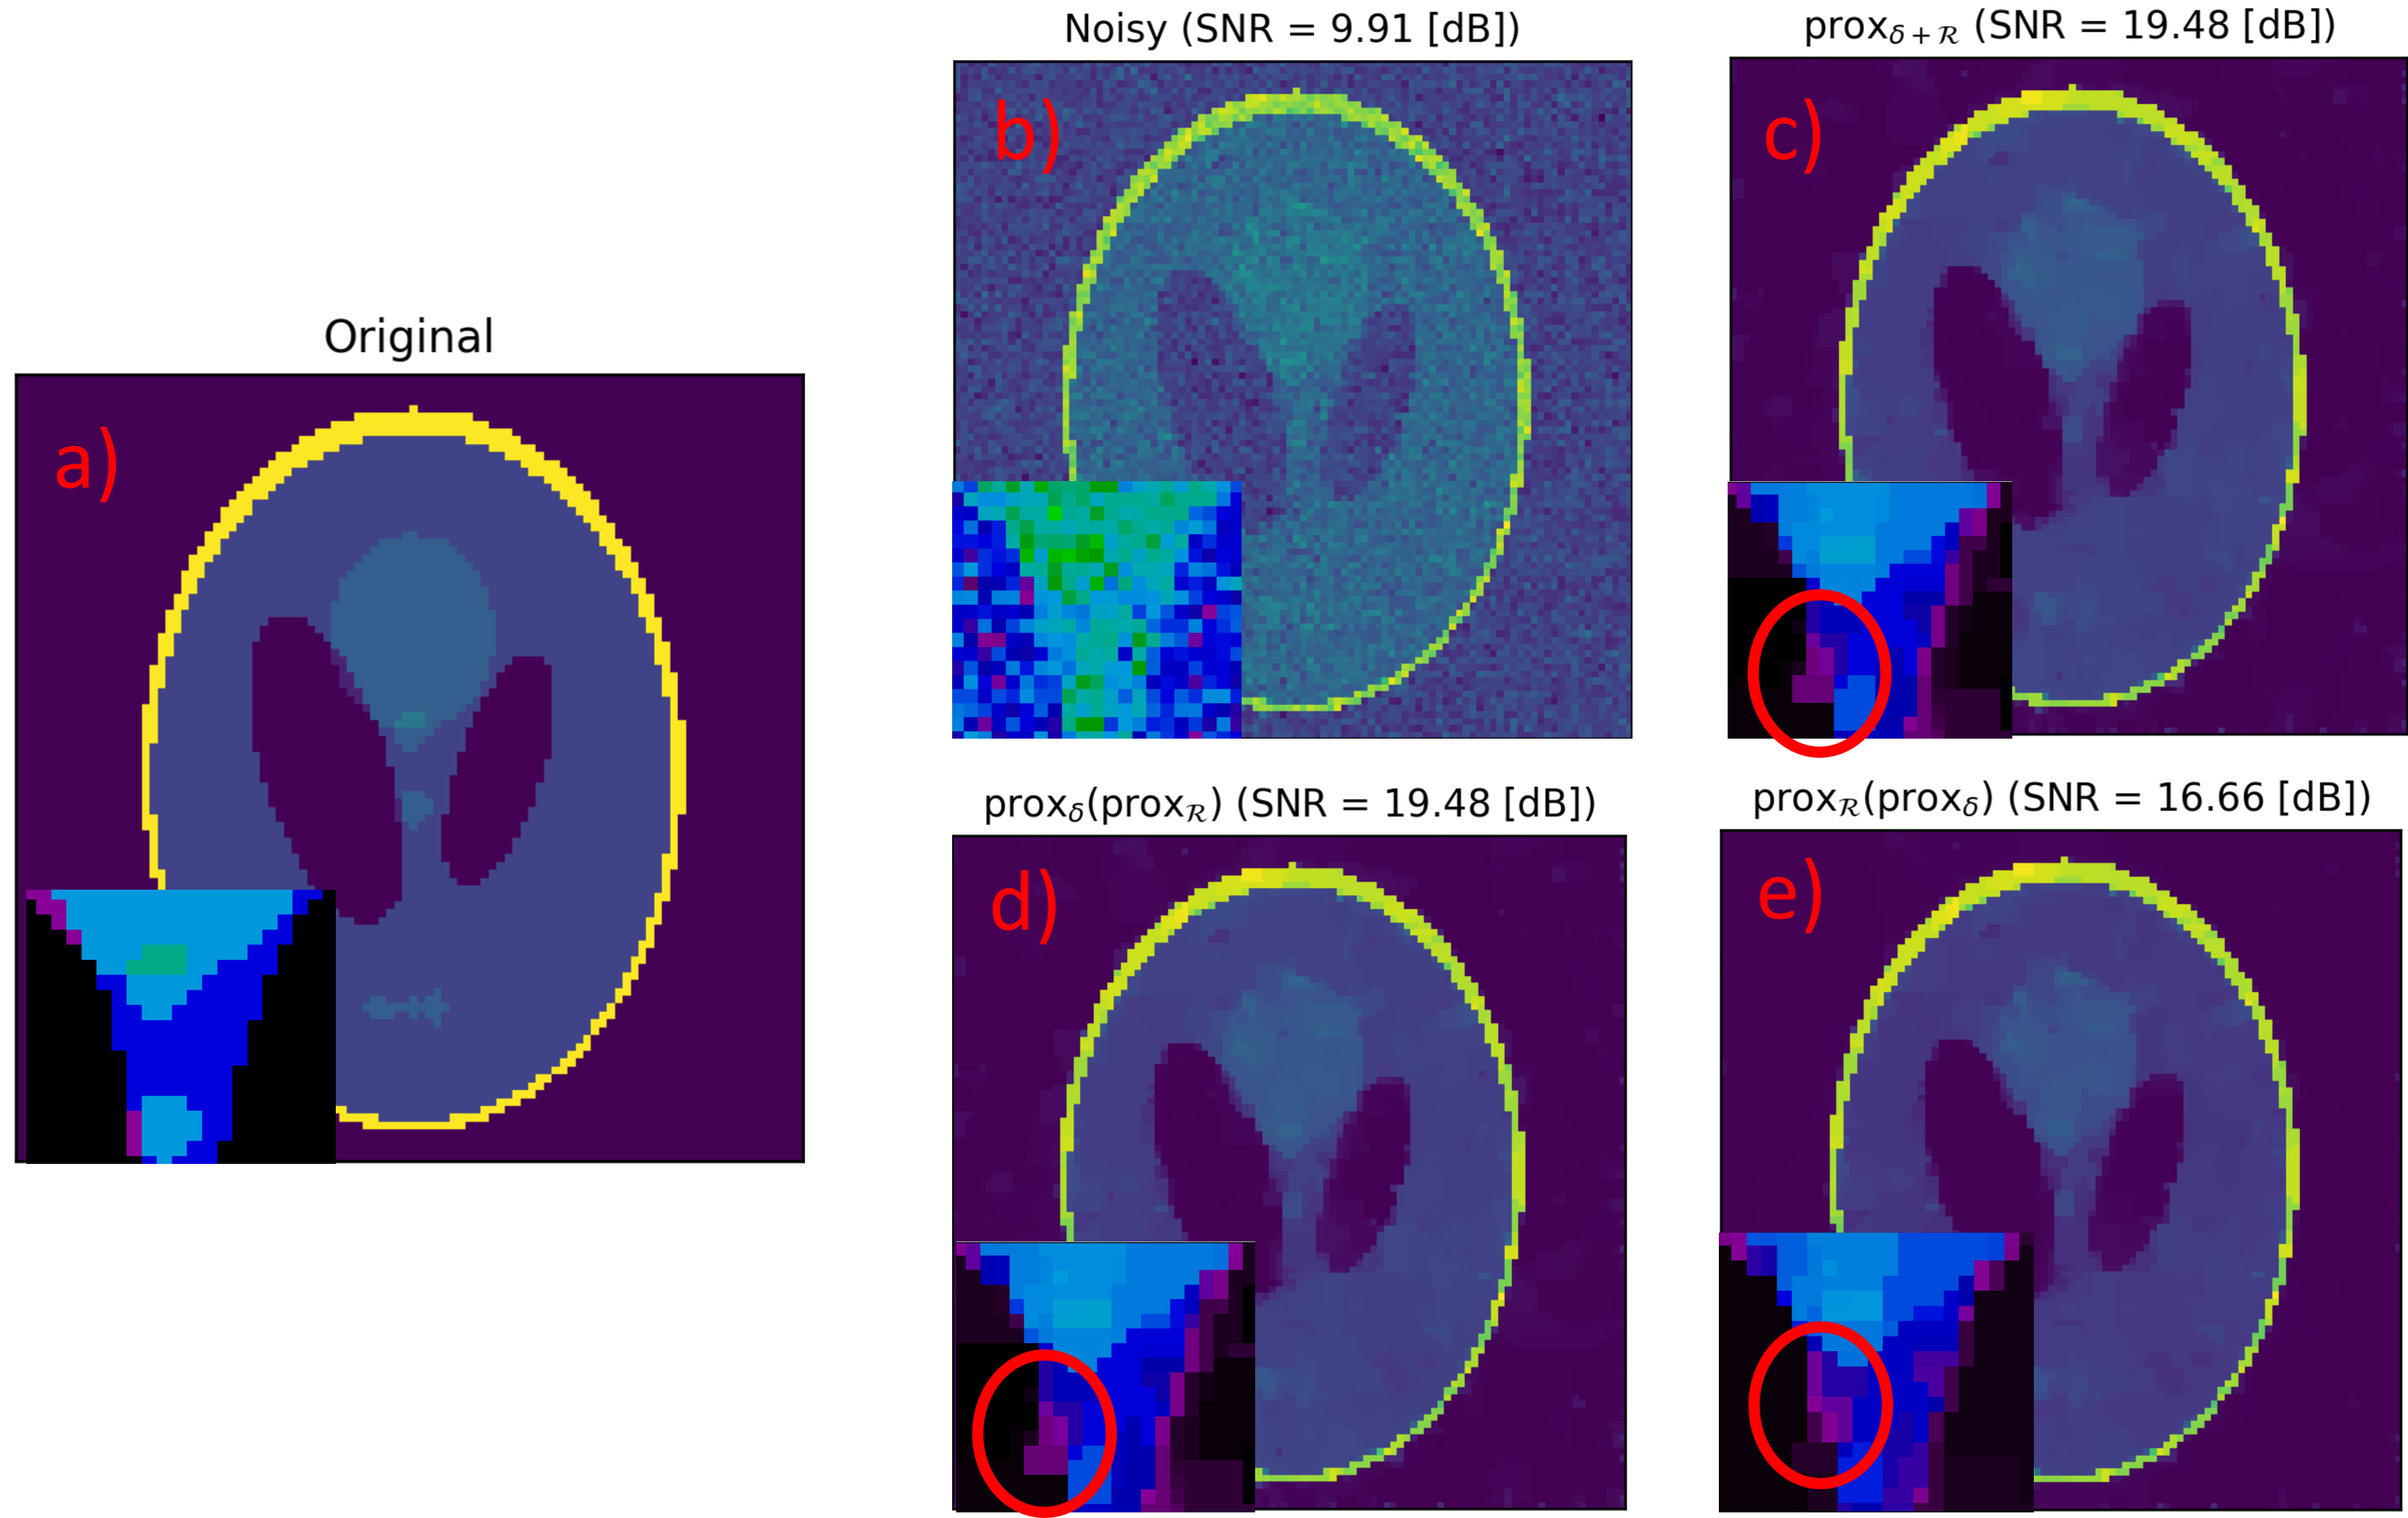
\includegraphics[scale = 0.6]{images/TV_experiments.png}
  \caption{Results of Total Variaton with nonnegativity constraints regularization on the Shepp Logan Phantom with Gaussian noise. a) shows original image, b) with Gaussian noise added, c) $\mathrm{prox}_{\mathcal{R} + \delta_{\rm \mathbb{R}_+^N}}(\mathbf{v})$ (ground truth), d) $\mathrm{prox}_{\delta_{\rm \mathbb{R}_+^N}}(\mathrm{prox}_{\mathcal{R}}(\mathbf{v}))$ (found in experiments -see table \ref{tab:exp_results}- to be equal to c), and e) $\mathrm{prox}_{\mathcal{R}}(\mathrm{prox}_{\delta_{\rm \mathbb{R}_+^N}}(\mathbf{v}))$. In each of the images, the center region is zoomed-in, to show some of the errors. Moreover, the $\mathrm{SNR}$ is shown in $\operatorname{[dB]}$.}
  \label{fig:tv_experiment}
  \end{center}
\end{figure}

In Figure \ref{fig:tv_experiment} we can see \eqref{eq:prox_nonneg(prox_r)} and \eqref{eq:prox_r(prox_nonneg)} applied to a real image. The original image was set to a size of $128 \times 128$, and normalized to the range $[0, 1]$. The added noise was sampled from the distribution $\mathcal{N}(0, 0.08)$. Just as in the random array scenario (see Table \ref{tab:exp_results}), between figures \ref{fig:tv_experiment}c) and \ref{fig:tv_experiment}d) there is an average absolute error in the order of $10^{-7}$, and the maximum absolute error is in the order of $10^{-5}$. Moreover, both visual inspection (see zoomed-in region for detailed zones) and $\mathrm{SNR}$ in $\operatorname{[dB]}$ show that both results are equal (and that there are indeed some differences between \ref{fig:tv_experiment}c) and \ref{fig:tv_experiment}e)). This promising result, that to the best of our knowledge is previously unknown, encourages the investigation of a closed-form solution of $\mathrm{prox}_{\operatorname{TV} + \delta_{\rm \mathbb{R}_+^N}}(\mathbf{v})$  and $\mathrm{prox}_{\operatorname{TV}}(\mathrm{prox}_{\delta_{\rm \mathbb{R}_+^N}}(\mathbf{v}))$, as well as the use of this result in image reconstruction libraries, as it has the potential to speed up image reconstruction.  

\noindent\textbf{Hessian-Schatten Norm}

For evaluation of the Hessian Schatten Norm, as for the evaluation of the simple Schatten norm, the results are not compelling enough to jump to a conclusion, and further investigation is required. Moreover, there are several technical constraints that hinder the proper evaluation of the Hessian Schatten Norm using CVXPy. As aforementioned, larger arrays with a higher $\sigma$ seem to have slightly more exact results, but the computational requirements of evaluating the Hessian-Schatten Norm make it unfeasible to evaluate bigger arrays than the ones presented in table \ref{tab:exp_results}. So while the results presented do not completely rule out the Hessian-Schatten norm for reduced splitting, a more efficient evaluation of the proximal operator of the Hessian-Schatten norm with nonnegativity constraints (an evaluation of the Hessian Schatten norm is presented in \cite{lefkimmiatis_poisson_2013}) is required to test for reduced splitting. 

For further evaluation, I performed an experiment on the standard test image \texttt{peppers}. The image was first normalized to the range $[0, 1]$, transformed to have a size of $64\times 64$ and finally had Gaussian noise added, sampled from $\mathcal{N}(0, 0.1)$. Regularization was done with $p=1$, which is the nuclear norm. The results are shown on figure \ref{fig:hs_experiment}
\begin{figure}[H]
  \begin{center}
  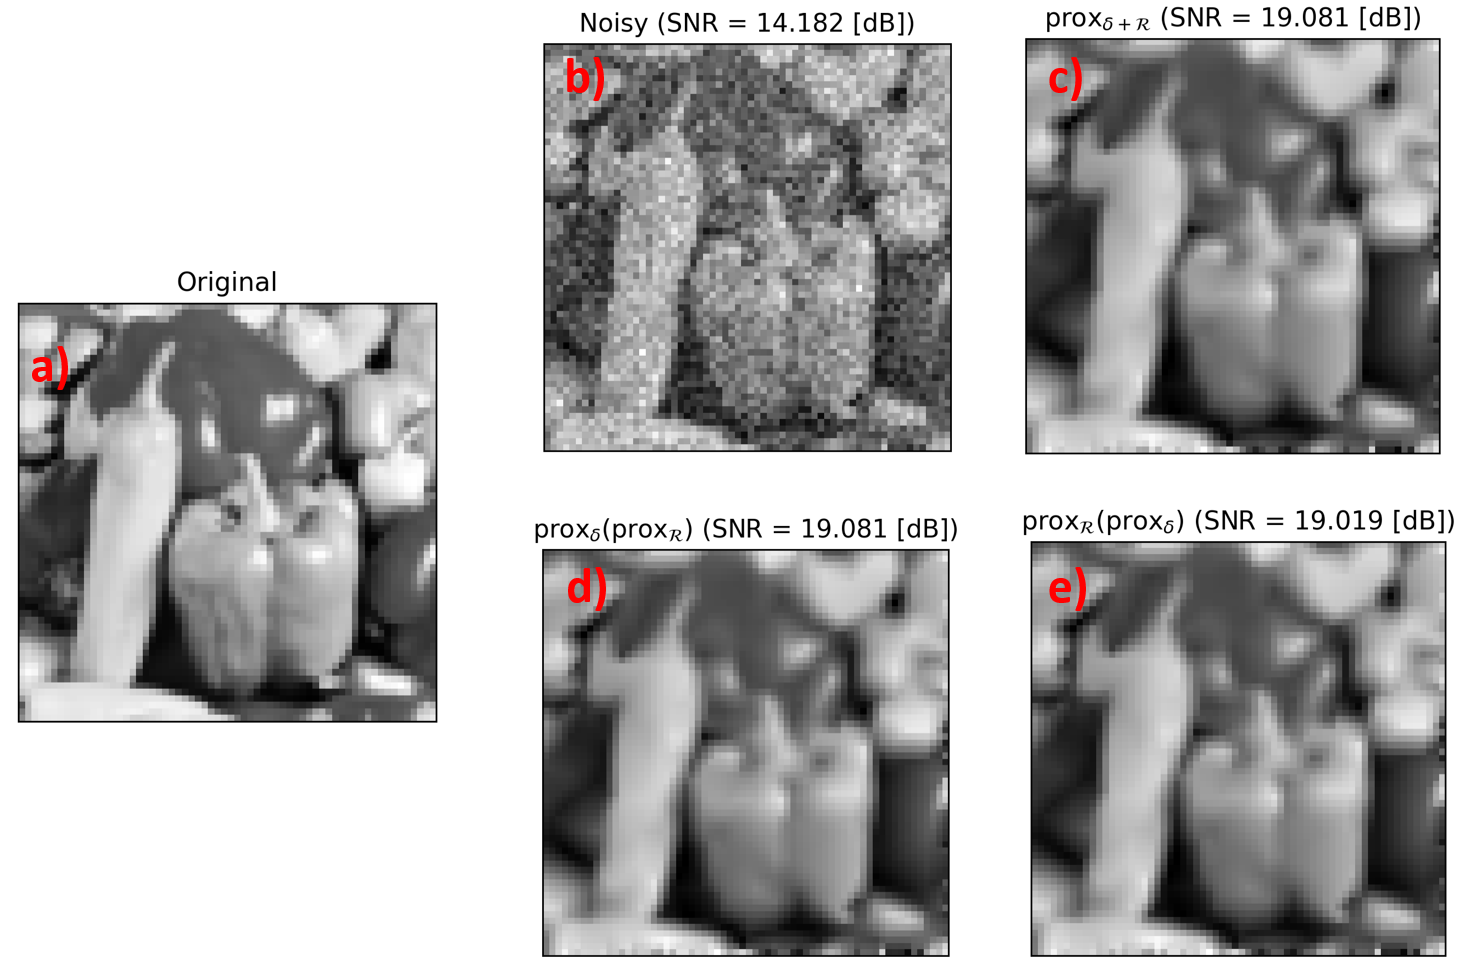
\includegraphics[scale = 0.6]{images/Peppers_experiment.png}
  \caption{Results of Hessian-Schatten norm with nonnegativity constraints regularization on standard \textit{Peppers} image with added Gaussian noise. a) shows original image in the range $[0, 1]$, b) with Gaussian noise added, sampled from $\mathcal{N}(0, 0.1)$, c) $\mathrm{prox}_{\mathcal{R} + \delta_{\rm \mathbb{R}_+^N}}(\mathbf{v})$ (ground truth), d) $\mathrm{prox}_{\delta_{\rm \mathbb{R}_+^N}}(\mathrm{prox}_{\mathcal{R}}(\mathbf{v}))$, and e) $\mathrm{prox}_{\mathcal{R}}(\mathrm{prox}_{\delta_{\rm \mathbb{R}_+^N}}(\mathbf{v}))$. Moreover, the \textit{SNR} is shown in \textit{dB}.}
  \label{fig:hs_experiment}
  \end{center}
\end{figure}

The results of the experiment on a standard test image, shown on Figure \ref{fig:hs_experiment} show the effectiveness of Hessian-Schatten norm regularization for denoising. Moreover, the experiment encourages the investigation of equation \eqref{eq:prox_nonneg(prox_r)}, as the maximum error between images \ref{fig:hs_experiment}c) and \ref{fig:hs_experiment}d) -that is, the left-hand and right-hand sides of \eqref{eq:prox_nonneg(prox_r)}- is in the order of $10^{-6}$, and the \textit{SNR} in $[\mathrm{dB}]$ is the same up to the $6^{\mathrm{th}}$ digit. On the other hand, the maximum error between images \ref{fig:hs_experiment}c) and \ref{fig:hs_experiment}e) is in the order of $10^{-2}$. While this error is not highly visible in the image, it does rule out \eqref{eq:prox_r(prox_nonneg)}. 

While the results of the experiment are encouraging, they are by no means compelling enough, as this experiment is just $1$, out of the $100$ (sampled from different distributions) that are used for the results presented in table \ref{tab:exp_results}. For further exploration, the same kind of experiment can be carried out by evaluating the proximal operator of the regularizer, instead of using a numerical approximation, as done here.  
